% !TeX root = ../../libro.tex
% !TeX encoding = utf8

A continuación se enuncian los ``hechos'' utilizados para las demostraciones de los teoremas. Su demostración detallada en varios casos se escapa de los límites del proyecto, en cuyos casos se aportarán demostraciones que suponen ciertos aquellos elementos propios de la teoría de Morse.

\begin{hecho}
	Todo $W \subset \R^2$ abierto tiene una triangulación clásica tal que el diámetro euclídeo de los triángulos se aproxima a $0$ en la frontera topológica de $W$.
\end{hecho}

\begin{proof}
	Tomamos la cuadrícula generada de forma natural por $\Z^2$ sobre $\R^2$. Vamos a definir de forma incremental el conjunto de cuadrados que cubren todo $W$.\\
	\\ Tomamos primero todos los cuadrados (cerrados) que estén contenidos estrictamente en $W$. Vamos a llamar $U$ a la parte cubierta por el conjunto de cuadrados actual.\\
	\\ Dado un $p \in W$ y $p \not \in U$ entonces existe un cuadrado que lo contiene pero que no está contenido estrictamente en $W$. Por ser $W$ abierto sabemos que para $p$ existe una bola abierta $B \subset W$ que lo contiene. De forma equivalente podemos subdividir el cuadrado inicial en $4$ cuadrados iguales, $8$ ... y así sucesivamente hasta encontrar una subdivisión en la que algún cuadrado contenga a $p$ y sea lo suficientemente pequeño como para que esté contenido en la bola $B \subset W$. Añadimos al conjunto todos los cuadrados anteriores que estén contenidos en $W$. Realizamos esta operación de manera indefinida.\\
	\\ Una vez definido el conjunto de cuadrados, podemos definir la triangulación como los triángulos resultantes de dividir por la diagonal dichos cuadrados. De esta forma tenemos una triangulación $T$ tal que la unión de sus triángulos, $U$, está contenida en $W$ pero todo punto $p \in W$ está en algún triángulo, por lo que $U = W$. Además, cuando tomamos $p$ tendiendo a $\partial W$, la bola $B \subset W$ que lo contiene tiene radio $\epsilon$ tendiendo a $0$, es decir, el cuadrado necesario para cubrirlo correctamente tiende a $0$, y como consecuencia los dos triángulos de los que se compone también.
\end{proof}

\begin{hecho}
	Toda variedad diferenciable $S$ tiene una triangulación diferenciable.
\end{hecho}

\begin{proof}
	Vamos a contruir una malla de polígonos diferenciables, que nos dará paso de forma trivial a una malla de triángulos diferenciables.\\
	\\ Podemos tomar $f:S \rightarrow \R$ función de Morse apropiada, es decir, los inversos de compactos son compactos y todos sus puntos críticos están a distintos niveles (es posible porque están aislados). Cortamos $S$ por los niveles de puntos no críticos, para separar los puntos críticos entre sí, obteniendo así una descomposición de $S$ en piezas difeomorfas a:
	\begin{itemize}
		\item Discos, tiene un punto crítico de orden $0$ o $2$.
		\item Anillos, no tiene puntos críticos.
		\item ``Pantalones'', o de forma equivalente, medio toro al que se le ha quitado un disco en el interior. Tiene un punto crítico de orden $1$.
		\item ``Pantalones cruzados'', o también se pueden ver como medio toro suma conexa con un espacio proyectivo $\mathbb{RP}^2$. Por ello, se puede dividir en unos ``pantalones'' normales y una cinta de Möbius. Tiene un punto crítico de orden $1$.
	\end{itemize} 
	
	Por la teoría de Morse tenemos una división de $S$ en conjuntos difeomorfos a alguno de los anteriores, todos ellos pegados por circunferencias (los bordes de los conjuntos descritos). Podemos obtener una malla añadiendo un vértice a cada circunferencia y seguidamente si es:
	\begin{itemize}
		\item Un disco, se toma el centro y se divide el disco en $3$ partes, teniendo $3$ sectores difeomorfos a un triángulo.
		\item Un anillo, se unen los $2$ vértices (uno de cada circunferencia del borde) mediante un arco, obteniendo así un cuadrilátero.
		\item Unos ``pantalones'', se unen los $3$ vértices mediante $2$ arcos (un vértice común a los $2$ arcos), dando lugar a un heptágono.
		\item Una cinta de Möbius, se une el vértice con él mismo mediante un arco, el cual recorre la mitad de la cara de la cinta, obteniendo así un triángulo.
	\end{itemize} 
	
	Finalmente tenemos la malla de polígonos diferenciables, la cual podemos convertir en una triangulación diferenciable dividiendo de forma adecuada los polígonos.
\end{proof}

\begin{hecho}
	Para toda estructura diferenciable $E$ del toro punteado $T'_E$ existe un subconjunto compacto suyo cuyo complemento es difeomorfo a $S^1 \times \R$ con la estructura diferenciable usual.
\end{hecho}

\begin{proof}
	Dividimos $T_S'$ tal y como lo hicimos en el $\textbf{Hecho 2.2}$, obteniendo así que está formado por piezas $P_j$ separadas por circunferencias $C_j$. Las piezas pueden ser discos, anillos o pantalones (cintas de Möbius no puesto que $T_S'$ es orientable y la orientabilidad es una propiedad topológica).\\
	\\ La forma en la que se pegan esas piezas $P_j$, se asocia a un grafo $G$ donde los vértices representan a cada $P_j$ y las aristas indican adyacencia (existe un $C_j$ entre las piezas que representan los vértices). Existe una aplicación cociente $q: T_S' \rightarrow G$ que lleva cada punto del entorno de una circunferencia $C_j$ a la correspondiente proyección sobre el arco de $G$ que representa a $C_j$. Por consiguiente, los $C_j$ van a los vértices del grafo $G$.\\

\begin{figure}[h]
  	\centering
  	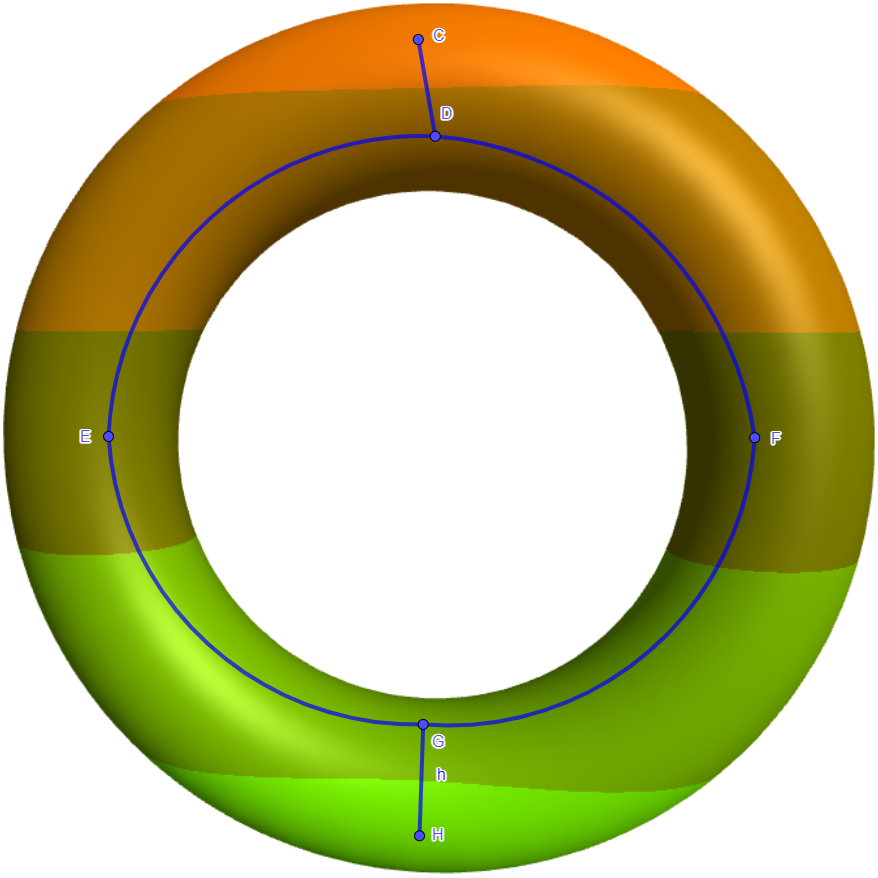
\includegraphics[width=0.4\textwidth]{grafo_asociado}
	\caption{Ejemplo de grafo asociado para la función de Morse ``altura'' que parte del Toro.}
  	\label{fig:grafo}
\end{figure}
	\newpage
	La aplicación $q_*:\Pi_1(T_S') \rightarrow \Pi_1(G)$ es un homomorfismo sobreyectivo con inversa a la izquierda, viendo $q$ como una homotopía. Por tanto, $\Pi_1(G)$ es un cociente de $\Pi_1(T_S')$, por lo que está finitamente generado. Esto implica que existe un subgrafo $G_0 \subset G$ tal que la clausura de $G - G_0$ consiste en un número finito de árboles ($G$ se puede retraer a $G_0$). Sólo uno de esos árboles puede no ser compacto puesto que a $T_S'$ le falta un único punto. Además, el no ser compacto implica que ese árbol está compuesto por un subárbol homeomorfo a $[0, \infty)$ junto con subárboles finitos pegados a él.\\
	\\ Podemos eliminar estos árboles finitos quitando las circunferencias que corresponden a dichos segmentos, cuyos vértices están asociados a discos $P_j$. Estas simplificaciones en $G$ se pueden ver como simplificaciones en la función de Morse entendiendo los $C_j$ como curvas de nivel, cancelando ``sillines''  con extremos locales (si es un disco que se adhiere a unos ``pantalones'') y anillos (si un $C_j$ separa un anillo de un disco). \\
	\\ Finalmente tenemos que $G$ tiene un subárbol no compacto $G_f$, homeomorfo a $[0, \infty)$ y la única posibilidad es que los segmentos correspondan a anillos, debido a que a $T_S'$ sólo le falta un punto, que se puede entender como el límite de dicha sucesión de $P_j$ y $C_j$. Tenemos que existe un compacto (la unión de los $P_j$ y $C_j$ correspondientes a $G - G_f$) cuyo complementario (los correspondientes a $G_f$) es una sucesión de anillos ``pegados'' de forma diferenciable en el sentido usual y por tanto es difeomorfo al cilindro con la estructura usual.
\end{proof}

\begin{hecho}
	Toda estructura diferenciable $E$ del toro $(S^1 \times S^1)_E$ es difeomorfa a la estructura usual del toro $S^1 \times S^1$.
\end{hecho}

\begin{proof}
	Partiendo de la demostración del hecho anterior, el grafo asociado $G$ ahora es finito con $\Pi_1(G)$ el cociente del grupo abeliano $\Pi_1(T_S)$, es decir, necesariamente $\Pi_1(G) = \Z$. Podemos reducir $G$ a una circunferencia, retrayendo los árboles finitos tal y como se hizo en la demostración anterior y haciendo los cambios necesarios en la función de $Morse$. La única posibilidad es que $T_S$ sea una sucesión de anillos pegados diferenciablemente, así que $T_S$ es difeomorfo a $T$ con la estructura usual o a una botella de Klein, pero no puede ser éste último por ser $\Pi_1(T_S)$ abeliano (ya que el grupo fundamental de la botella de Klein no es abeliano y no es posible siquiera un homeomorfismo entre ellos).
\end{proof}

\begin{hecho}
	Sea $E$ una estructura diferenciable en $D^1 \times \R$ tal que es la usual en un entorno del borde. Entonces existe un difeomorfismo $g:(D^1 \times \R)_E \rightarrow (D^1 \times \R)_U$, con $U$ la estructura usual, que además es la identidad entorno a $\partial D^1 \times \R$.
\end{hecho}

\begin{proof}
	Tomamos la proyección $\pi : (D^1 \times \R)_S \rightarrow \R$ que ya es diferenciable en un entorno del borde. Si vemos $(D^1 \times \R)_{S}$ como una variedad sabemos que existe una  función de Morse $f : (D^1 \times \R)_S \rightarrow \R$, a la que podemos obligar que coincida con $|\pi$ en un entorno del borde más pequeño que en el que es diferenciable $\pi$, donde no tendrá puntos críticos. \\
	\\ La función $f$ es una función de Morse propia, con todos sus puntos críticos en distintos niveles. Los niveles de puntos no críticos están formados por un único arco y una o varias circunferencias. Al cortar por dichos niveles obtenemos discos, anillos, ``pantalones'', rectángulos y rectángulos con un ``agujero'' (un rectángulo menos un disco abierto). El grafo asociado $G$ es un árbol debido a que $\Pi_1(D^1 \times \R) = 0$, y procedemos como en la demostración del hecho $2.3$, alterando $f$ de forma que el $G$ asociado sea homeomorfo a $\R$. \\
	\\ La nueva función $f$ no tiene puntos críticos, por lo que puede ser la segunda componente de un difeomorfismo $g:(D^1 \times \R)_S \rightarrow D^1 \times \R$, que coincidirá con la identidad en un entorno del borde. La primera componente se puede obtener a partir del campo de vectores gradientes de $f$, de forma similar a como se prosigue en la demostración del teorema $2.2$ de la teoría de Morse.
\end{proof}

\begin{hecho}
	Sea $E$ una estructura diferenciable en $D^2$ tal que es la usual en un entorno del borde. Entonces existe un difeomorfismo $g:D^2_E \rightarrow D^2_U$, con $U$ la estructura usual, que además es la identidad entorno a $\partial D^2$.
\end{hecho}

\begin{proof}
	Tomamos la función que devuelve el radio (distancia al origen) en un entorno de $\partial D^2_S$ y como es diferenciable, la extendemos a una función de Morse propia $f:D^2_S \rightarrow (0,1]$, cuyos puntos críticos están en el interior y $f^{-1}(1) = \partial D^2_S$.\\
	\\ El grafo asociado $G$ es un árbol por ser $\Pi_1(D^2) = 0$ y deformando $f$ como se hizo anteriormente, podemos simplificar $G$  a un único punto. Entonces, $f$ sólo tiene un punto crítico $p$, que necesariamente debe de ser de índice $0$ porque coincide con la función ``radio'' en el borde ($f$ decrece a medida que nos acercamos $p$, es decir, en $p$ la matriz Hessiana es definida positiva y por tanto el índice es $0$).\\
	\\ Construimos $g:D^2_S \rightarrow D^2$ difeomorfismo a partir de $f$ de manera similar a como se hizo en el apartado anterior, reproduciendo parte de la demostración del teorema $2.2$ (siguiendo el flujo del campo de vectores gradientes de $f$). En particular, tenemos que $g$ es la identidad en un entorno de $\partial D^2_S$.
\end{proof}



\endinput
%------------------------------------------------------------------------------------
% FIN DEL CAPÍTULO. 
%------------------------------------------------------------------------------------
